% Options for packages loaded elsewhere
\PassOptionsToPackage{unicode}{hyperref}
\PassOptionsToPackage{hyphens}{url}
%
\documentclass[
  10pt,
]{article}
\usepackage{lmodern}
\usepackage{amsmath}
\usepackage{ifxetex,ifluatex}
\ifnum 0\ifxetex 1\fi\ifluatex 1\fi=0 % if pdftex
  \usepackage[T1]{fontenc}
  \usepackage[utf8]{inputenc}
  \usepackage{textcomp} % provide euro and other symbols
  \usepackage{amssymb}
\else % if luatex or xetex
  \usepackage{unicode-math}
  \defaultfontfeatures{Scale=MatchLowercase}
  \defaultfontfeatures[\rmfamily]{Ligatures=TeX,Scale=1}
\fi
% Use upquote if available, for straight quotes in verbatim environments
\IfFileExists{upquote.sty}{\usepackage{upquote}}{}
\IfFileExists{microtype.sty}{% use microtype if available
  \usepackage[]{microtype}
  \UseMicrotypeSet[protrusion]{basicmath} % disable protrusion for tt fonts
}{}
\makeatletter
\@ifundefined{KOMAClassName}{% if non-KOMA class
  \IfFileExists{parskip.sty}{%
    \usepackage{parskip}
  }{% else
    \setlength{\parindent}{0pt}
    \setlength{\parskip}{6pt plus 2pt minus 1pt}}
}{% if KOMA class
  \KOMAoptions{parskip=half}}
\makeatother
\usepackage{xcolor}
\IfFileExists{xurl.sty}{\usepackage{xurl}}{} % add URL line breaks if available
\IfFileExists{bookmark.sty}{\usepackage{bookmark}}{\usepackage{hyperref}}
\hypersetup{
  pdftitle={EDDA - Assignment 2 - Group 77},
  hidelinks,
  pdfcreator={LaTeX via pandoc}}
\urlstyle{same} % disable monospaced font for URLs
\usepackage[margin=1in]{geometry}
\usepackage{color}
\usepackage{fancyvrb}
\newcommand{\VerbBar}{|}
\newcommand{\VERB}{\Verb[commandchars=\\\{\}]}
\DefineVerbatimEnvironment{Highlighting}{Verbatim}{commandchars=\\\{\}}
% Add ',fontsize=\small' for more characters per line
\usepackage{framed}
\definecolor{shadecolor}{RGB}{248,248,248}
\newenvironment{Shaded}{\begin{snugshade}}{\end{snugshade}}
\newcommand{\AlertTok}[1]{\textcolor[rgb]{0.94,0.16,0.16}{#1}}
\newcommand{\AnnotationTok}[1]{\textcolor[rgb]{0.56,0.35,0.01}{\textbf{\textit{#1}}}}
\newcommand{\AttributeTok}[1]{\textcolor[rgb]{0.77,0.63,0.00}{#1}}
\newcommand{\BaseNTok}[1]{\textcolor[rgb]{0.00,0.00,0.81}{#1}}
\newcommand{\BuiltInTok}[1]{#1}
\newcommand{\CharTok}[1]{\textcolor[rgb]{0.31,0.60,0.02}{#1}}
\newcommand{\CommentTok}[1]{\textcolor[rgb]{0.56,0.35,0.01}{\textit{#1}}}
\newcommand{\CommentVarTok}[1]{\textcolor[rgb]{0.56,0.35,0.01}{\textbf{\textit{#1}}}}
\newcommand{\ConstantTok}[1]{\textcolor[rgb]{0.00,0.00,0.00}{#1}}
\newcommand{\ControlFlowTok}[1]{\textcolor[rgb]{0.13,0.29,0.53}{\textbf{#1}}}
\newcommand{\DataTypeTok}[1]{\textcolor[rgb]{0.13,0.29,0.53}{#1}}
\newcommand{\DecValTok}[1]{\textcolor[rgb]{0.00,0.00,0.81}{#1}}
\newcommand{\DocumentationTok}[1]{\textcolor[rgb]{0.56,0.35,0.01}{\textbf{\textit{#1}}}}
\newcommand{\ErrorTok}[1]{\textcolor[rgb]{0.64,0.00,0.00}{\textbf{#1}}}
\newcommand{\ExtensionTok}[1]{#1}
\newcommand{\FloatTok}[1]{\textcolor[rgb]{0.00,0.00,0.81}{#1}}
\newcommand{\FunctionTok}[1]{\textcolor[rgb]{0.00,0.00,0.00}{#1}}
\newcommand{\ImportTok}[1]{#1}
\newcommand{\InformationTok}[1]{\textcolor[rgb]{0.56,0.35,0.01}{\textbf{\textit{#1}}}}
\newcommand{\KeywordTok}[1]{\textcolor[rgb]{0.13,0.29,0.53}{\textbf{#1}}}
\newcommand{\NormalTok}[1]{#1}
\newcommand{\OperatorTok}[1]{\textcolor[rgb]{0.81,0.36,0.00}{\textbf{#1}}}
\newcommand{\OtherTok}[1]{\textcolor[rgb]{0.56,0.35,0.01}{#1}}
\newcommand{\PreprocessorTok}[1]{\textcolor[rgb]{0.56,0.35,0.01}{\textit{#1}}}
\newcommand{\RegionMarkerTok}[1]{#1}
\newcommand{\SpecialCharTok}[1]{\textcolor[rgb]{0.00,0.00,0.00}{#1}}
\newcommand{\SpecialStringTok}[1]{\textcolor[rgb]{0.31,0.60,0.02}{#1}}
\newcommand{\StringTok}[1]{\textcolor[rgb]{0.31,0.60,0.02}{#1}}
\newcommand{\VariableTok}[1]{\textcolor[rgb]{0.00,0.00,0.00}{#1}}
\newcommand{\VerbatimStringTok}[1]{\textcolor[rgb]{0.31,0.60,0.02}{#1}}
\newcommand{\WarningTok}[1]{\textcolor[rgb]{0.56,0.35,0.01}{\textbf{\textit{#1}}}}
\usepackage{longtable,booktabs}
\usepackage{calc} % for calculating minipage widths
% Correct order of tables after \paragraph or \subparagraph
\usepackage{etoolbox}
\makeatletter
\patchcmd\longtable{\par}{\if@noskipsec\mbox{}\fi\par}{}{}
\makeatother
% Allow footnotes in longtable head/foot
\IfFileExists{footnotehyper.sty}{\usepackage{footnotehyper}}{\usepackage{footnote}}
\makesavenoteenv{longtable}
\usepackage{graphicx}
\makeatletter
\def\maxwidth{\ifdim\Gin@nat@width>\linewidth\linewidth\else\Gin@nat@width\fi}
\def\maxheight{\ifdim\Gin@nat@height>\textheight\textheight\else\Gin@nat@height\fi}
\makeatother
% Scale images if necessary, so that they will not overflow the page
% margins by default, and it is still possible to overwrite the defaults
% using explicit options in \includegraphics[width, height, ...]{}
\setkeys{Gin}{width=\maxwidth,height=\maxheight,keepaspectratio}
% Set default figure placement to htbp
\makeatletter
\def\fps@figure{htbp}
\makeatother
\setlength{\emergencystretch}{3em} % prevent overfull lines
\providecommand{\tightlist}{%
  \setlength{\itemsep}{0pt}\setlength{\parskip}{0pt}}
\setcounter{secnumdepth}{-\maxdimen} % remove section numbering
\ifluatex
  \usepackage{selnolig}  % disable illegal ligatures
\fi

\title{EDDA - Assignment 2 - Group 77}
\usepackage{etoolbox}
\makeatletter
\providecommand{\subtitle}[1]{% add subtitle to \maketitle
  \apptocmd{\@title}{\par {\large #1 \par}}{}{}
}
\makeatother
\subtitle{Dante de Lang, Ignas Krikštaponis and Kamiel Gülpen}
\author{}
\date{\vspace{-2.5em}}

\begin{document}
\maketitle

\hypertarget{exercise-1}{%
\section{Exercise 1}\label{exercise-1}}

\textbf{a)}The 18 slices came from a single loaf, but were randomized to
the 6 combinations of conditions. Present an R-code for this
randomization process.

\begin{Shaded}
\begin{Highlighting}[]
\NormalTok{data\_bread }\OtherTok{\textless{}{-}} \FunctionTok{read.table}\NormalTok{(}\AttributeTok{file=}\StringTok{"data/bread.txt"}\NormalTok{, }\AttributeTok{header=}\ConstantTok{TRUE}\NormalTok{)}
\NormalTok{humid }\OtherTok{\textless{}{-}} \FunctionTok{factor}\NormalTok{(}\FunctionTok{rep}\NormalTok{(}\FunctionTok{c}\NormalTok{(}\StringTok{"dry"}\NormalTok{,}\StringTok{"wet"}\NormalTok{),}\AttributeTok{each =} \DecValTok{9}\NormalTok{))}
\NormalTok{temp }\OtherTok{\textless{}{-}} \FunctionTok{factor}\NormalTok{(}\FunctionTok{rep}\NormalTok{(}\FunctionTok{c}\NormalTok{(}\StringTok{"cold"}\NormalTok{, }\StringTok{"intermediate"}\NormalTok{,}\StringTok{"warm"}\NormalTok{), }\AttributeTok{times =} \DecValTok{6}\NormalTok{))}
\NormalTok{knitr}\SpecialCharTok{::}\FunctionTok{kable}\NormalTok{(}\FunctionTok{data.frame}\NormalTok{(humid,temp,}\AttributeTok{slice =} \FunctionTok{sample}\NormalTok{(}\DecValTok{1}\SpecialCharTok{:}\DecValTok{18}\NormalTok{)), }
             \AttributeTok{caption =} \StringTok{"Randomised combinations"}\NormalTok{)}
\end{Highlighting}
\end{Shaded}

\begin{longtable}[]{@{}llr@{}}
\caption{Randomised combinations}\tabularnewline
\toprule
humid & temp & slice\tabularnewline
\midrule
\endfirsthead
\toprule
humid & temp & slice\tabularnewline
\midrule
\endhead
dry & cold & 7\tabularnewline
dry & intermediate & 15\tabularnewline
dry & warm & 16\tabularnewline
dry & cold & 11\tabularnewline
dry & intermediate & 4\tabularnewline
dry & warm & 8\tabularnewline
dry & cold & 1\tabularnewline
dry & intermediate & 12\tabularnewline
dry & warm & 6\tabularnewline
wet & cold & 18\tabularnewline
wet & intermediate & 3\tabularnewline
wet & warm & 2\tabularnewline
wet & cold & 13\tabularnewline
wet & intermediate & 5\tabularnewline
wet & warm & 17\tabularnewline
wet & cold & 9\tabularnewline
wet & intermediate & 14\tabularnewline
wet & warm & 10\tabularnewline
\bottomrule
\end{longtable}

\textbf{b)}Make two boxplots of hours versus the two factors and two
interaction plots (keeping the two factors fixed in turn).

\begin{Shaded}
\begin{Highlighting}[]
\FunctionTok{par}\NormalTok{(}\AttributeTok{mfrow=}\FunctionTok{c}\NormalTok{(}\DecValTok{2}\NormalTok{,}\DecValTok{2}\NormalTok{))}
\FunctionTok{boxplot}\NormalTok{(data\_bread}\SpecialCharTok{$}\NormalTok{hours}\SpecialCharTok{\textasciitilde{}}\NormalTok{data\_bread}\SpecialCharTok{$}\NormalTok{environment)}
\FunctionTok{boxplot}\NormalTok{(data\_bread}\SpecialCharTok{$}\NormalTok{hours}\SpecialCharTok{\textasciitilde{}}\NormalTok{data\_bread}\SpecialCharTok{$}\NormalTok{humidity)}
\FunctionTok{interaction.plot}\NormalTok{(data\_bread}\SpecialCharTok{$}\NormalTok{humidity,data\_bread}\SpecialCharTok{$}\NormalTok{environment,data\_bread}\SpecialCharTok{$}\NormalTok{hours)}
\FunctionTok{interaction.plot}\NormalTok{(data\_bread}\SpecialCharTok{$}\NormalTok{environment,data\_bread}\SpecialCharTok{$}\NormalTok{humidity,data\_bread}\SpecialCharTok{$}\NormalTok{hours)}
\end{Highlighting}
\end{Shaded}

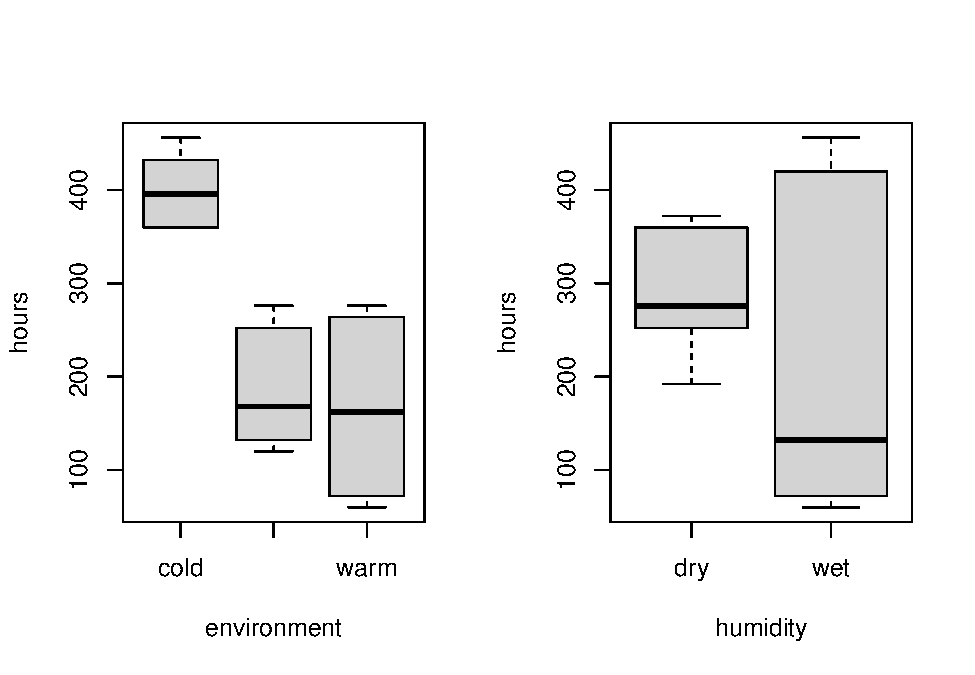
\includegraphics{Assignment-2_files/figure-latex/unnamed-chunk-2-1.pdf}

\textbf{c)}Perform an analysis of variance to test for effect of the
factors temperature, humidity, and the interaction. Describe the
interaction effect in words.

\begin{Shaded}
\begin{Highlighting}[]
\FunctionTok{attach}\NormalTok{(data\_bread)}
\NormalTok{environment}\OtherTok{=}\FunctionTok{as.factor}\NormalTok{(environment)}
\NormalTok{humidity}\OtherTok{=}\FunctionTok{as.factor}\NormalTok{(humidity)}
\NormalTok{dataaov}\OtherTok{=}\FunctionTok{lm}\NormalTok{(hours}\SpecialCharTok{\textasciitilde{}}\NormalTok{humidity}\SpecialCharTok{*}\NormalTok{environment,}\AttributeTok{data=}\NormalTok{data\_bread)}
\FunctionTok{anova}\NormalTok{(dataaov)}
\end{Highlighting}
\end{Shaded}

\begin{verbatim}
## Analysis of Variance Table
## 
## Response: hours
##                      Df Sum Sq Mean Sq F value  Pr(>F)    
## humidity              1  26912   26912    62.3 4.3e-06 ***
## environment           2 201904  100952   233.7 2.5e-10 ***
## humidity:environment  2  55984   27992    64.8 3.7e-07 ***
## Residuals            12   5184     432                    
## ---
## Signif. codes:  0 '***' 0.001 '**' 0.01 '*' 0.05 '.' 0.1 ' ' 1
\end{verbatim}

\begin{Shaded}
\begin{Highlighting}[]
\FunctionTok{summary}\NormalTok{(dataaov)}\SpecialCharTok{$}\NormalTok{coefficients}
\end{Highlighting}
\end{Shaded}

\begin{verbatim}
##                                     Estimate Std. Error t value Pr(>|t|)
## (Intercept)                              364         12   30.33 1.03e-12
## humiditywet                               72         17    4.24 1.14e-03
## environmentintermediate                 -124         17   -7.31 9.39e-06
## environmentwarm                         -100         17   -5.89 7.34e-05
## humiditywet:environmentintermediate     -180         24   -7.50 7.23e-06
## humiditywet:environmentwarm             -268         24  -11.17 1.07e-07
\end{verbatim}

When looking at the two-way anova model we see that it consists of the
following terms: \(Y_{ijk}\) = \(\mu_{ij}\) + \(e_{ijk}\) =
\(\mu + alpha_{i}\) + \(\beta_{j}\) + \(\gamma_{ij}\) + \(e_{eijk}\) We
decompose the formula in this way such that \(\mu\) is the overall mean,
\(\alpha_{i}\) and \(\beta_{j}\) are the main effect of level i and j of
the first factor and second factor respectively and \(\gamma_{ij}\) the
interaction effect.

In order to test the effect of the temperature, humidity and the
interaction we set up 3 hypotheses which are: \(H_{AB}\):
\(\gamma_{ij}\) = 0 for every (i, j) (no interactions between factor A
and B)

\(H_{A}\): \(\alpha_{i}\) = 0 for every i (no main effect of factor A)

\(H_{B}\):\(\beta_{j}\) = 0 for every j (no main effect of factor B)

We use the test statistics \(F_{AB}\) for \(H_{AB}\), \(F_{A}\) for
\(H_{A}\) and \(F_{B}\) for \(H_{B}\) where F is the F-distribution.

To see if the Hypotheses can be rejected we want to look at the
probability that P(F\textgreater{}\(f_{AB}\)),
P(F\textgreater{}\(f_{A}\)) and P(F\textgreater{}\(f_{B}\)), the bigger
the F value the lower the probability that the Hypothesis lays under a
F-distribution and therefore the Hypothesis can be rejected.

We see that the humidity has a p-value of 4.3e-06, environment a p-value
of 2.5e-10 and the interaction between the two (humidity:environment)
shows a p-value of 3.7e-07. This means that humidity, environment and
the interaction effect between humidity and environment have a
significant influence on the hours, which means we can reject \(H_{A}\),
\(H_{B}\) and \(H_{AB}\).

The interaction effect looks at the difference of differences, for
example: it looks at the difference in hours for environment = cold and
environment = warm for humidity = wet. Then it looks at the difference
between environment = cold and environment = warm for humidity = dry. It
then looks at the difference between those differences and when this
difference is high it shows that there is indeed interaction.

\textbf{d)} Which of the two factors has the greatest (numerical)
influence on the decay? Is this a good question?

To answer this question we would need to construct an additive model.
However, in \(c)\) we concluded that there is significant interaction
between the two factors, therefore, it is not proper to simply decompose
the effects of the two factors with the additive model - the question is
not correct.

\textbf{e)} Check the model assumptions by using relevant diagnostic
tools. Are there any outliers?

\begin{Shaded}
\begin{Highlighting}[]
\FunctionTok{par}\NormalTok{(}\AttributeTok{mfrow=}\FunctionTok{c}\NormalTok{(}\DecValTok{1}\NormalTok{,}\DecValTok{2}\NormalTok{))}
\NormalTok{dataaov2}\OtherTok{=}\FunctionTok{lm}\NormalTok{(hours}\SpecialCharTok{\textasciitilde{}}\NormalTok{humidity}\SpecialCharTok{*}\NormalTok{environment,}\AttributeTok{data=}\NormalTok{data\_bread); }
\FunctionTok{plot}\NormalTok{(dataaov2, }\DecValTok{1}\NormalTok{)}
\FunctionTok{plot}\NormalTok{(dataaov2, }\DecValTok{2}\NormalTok{)}
\end{Highlighting}
\end{Shaded}

\includegraphics{Assignment-2_files/figure-latex/unnamed-chunk-4-1.pdf}
The qqplot shows a somewhat linear line which means we can conclude that
the data is normally distributed - however, there are some outliers at
the extremes marked with 5, 7 and 8. We also looked at the Residuals vs
Fitted plot, which showed no obvious relationship - which is an
acceptable behavior.

\hypertarget{exercise-2}{%
\section{Exercise 2}\label{exercise-2}}

\textbf{a)} Number the selected students 1 to 15 and show how (by using
R) the students could be randomized to the interfaces in a randomized
block design.

\begin{Shaded}
\begin{Highlighting}[]
\NormalTok{interface }\OtherTok{\textless{}{-}} \FunctionTok{factor}\NormalTok{(}\FunctionTok{rep}\NormalTok{(}\FunctionTok{c}\NormalTok{(}\DecValTok{1}\NormalTok{,}\DecValTok{2}\NormalTok{,}\DecValTok{3}\NormalTok{),}\AttributeTok{each =} \DecValTok{5}\NormalTok{))}
\NormalTok{skill }\OtherTok{\textless{}{-}} \FunctionTok{factor}\NormalTok{(}\FunctionTok{rep}\NormalTok{(}\FunctionTok{c}\NormalTok{(}\DecValTok{1}\NormalTok{,}\DecValTok{2}\NormalTok{,}\DecValTok{3}\NormalTok{,}\DecValTok{4}\NormalTok{,}\DecValTok{5}\NormalTok{),}\AttributeTok{times =} \DecValTok{3}\NormalTok{))}
\NormalTok{student }\OtherTok{\textless{}{-}} \FunctionTok{sample}\NormalTok{(}\FunctionTok{c}\NormalTok{(}\DecValTok{1}\SpecialCharTok{:}\DecValTok{15}\NormalTok{))}
\NormalTok{knitr}\SpecialCharTok{::}\FunctionTok{kable}\NormalTok{(}\FunctionTok{data.frame}\NormalTok{(student,skill,interface), }\AttributeTok{caption =} \StringTok{"Randomised block design"}\NormalTok{)}
\end{Highlighting}
\end{Shaded}

\begin{longtable}[]{@{}rll@{}}
\caption{Randomised block design}\tabularnewline
\toprule
student & skill & interface\tabularnewline
\midrule
\endfirsthead
\toprule
student & skill & interface\tabularnewline
\midrule
\endhead
8 & 1 & 1\tabularnewline
5 & 2 & 1\tabularnewline
11 & 3 & 1\tabularnewline
13 & 4 & 1\tabularnewline
12 & 5 & 1\tabularnewline
15 & 1 & 2\tabularnewline
1 & 2 & 2\tabularnewline
10 & 3 & 2\tabularnewline
9 & 4 & 2\tabularnewline
14 & 5 & 2\tabularnewline
7 & 1 & 3\tabularnewline
2 & 2 & 3\tabularnewline
6 & 3 & 3\tabularnewline
3 & 4 & 3\tabularnewline
4 & 5 & 3\tabularnewline
\bottomrule
\end{longtable}

\textbf{b)} Test the null hypothesis that the search time is the same
for all interfaces. What type of interface does require the longest
search time? For which combination of skill level and type of interface
is the search time the shortest? Estimate the time it takes a typical
user of skill level 3 to find the product on the website if the website
uses interface 3.

\begin{Shaded}
\begin{Highlighting}[]
\NormalTok{data\_search }\OtherTok{\textless{}{-}} \FunctionTok{read.table}\NormalTok{(}\AttributeTok{file=}\StringTok{"data/search.txt"}\NormalTok{,}\AttributeTok{header=}\ConstantTok{TRUE}\NormalTok{)}
\NormalTok{data\_search}\SpecialCharTok{$}\NormalTok{skill }\OtherTok{\textless{}{-}} \FunctionTok{as.factor}\NormalTok{(data\_search}\SpecialCharTok{$}\NormalTok{skill)}
\NormalTok{data\_search}\SpecialCharTok{$}\NormalTok{interface }\OtherTok{\textless{}{-}} \FunctionTok{as.factor}\NormalTok{(data\_search}\SpecialCharTok{$}\NormalTok{interface)}
\CommentTok{\# perform ANOVA}
\NormalTok{aovsearch }\OtherTok{=} \FunctionTok{lm}\NormalTok{(time}\SpecialCharTok{\textasciitilde{}}\NormalTok{interface}\SpecialCharTok{+}\NormalTok{skill, }\AttributeTok{data=}\NormalTok{ data\_search);  }\FunctionTok{anova}\NormalTok{(aovsearch); }
\end{Highlighting}
\end{Shaded}

\begin{verbatim}
## Analysis of Variance Table
## 
## Response: time
##           Df Sum Sq Mean Sq F value Pr(>F)  
## interface  2   50.5   25.23    7.82  0.013 *
## skill      4   80.1   20.01    6.21  0.014 *
## Residuals  8   25.8    3.23                 
## ---
## Signif. codes:  0 '***' 0.001 '**' 0.01 '*' 0.05 '.' 0.1 ' ' 1
\end{verbatim}

\begin{Shaded}
\begin{Highlighting}[]
\FunctionTok{summary}\NormalTok{(aovsearch)}\SpecialCharTok{$}\NormalTok{coefficients }
\end{Highlighting}
\end{Shaded}

\begin{verbatim}
##             Estimate Std. Error t value Pr(>|t|)
## (Intercept)    15.01       1.23  12.238 1.85e-06
## interface2      2.70       1.14   2.377 4.47e-02
## interface3      4.46       1.14   3.927 4.38e-03
## skill2          1.30       1.47   0.887 4.01e-01
## skill3          3.03       1.47   2.069 7.24e-02
## skill4          5.30       1.47   3.614 6.84e-03
## skill5          6.10       1.47   4.160 3.16e-03
\end{verbatim}

Looking at the additive ANOVA test we can conclude that there is a
significant main effect of the interface (p-value \textless{} 0.05) -
therefore, the search times are not the same between the interfaces.
Furthermore, the summary shows that interface 3 gives the highest
\(\alpha\) parameter value, making search time the longest for this
interface type. For the shortest search time, interface 1 can be
combined with skill levels 1, 2 or 3 since all three have the lowest
\(\beta\) parameter values with 2 and 3 not being significantly
different from skill level 1. If significance is disregarded,
combination of interface 1 with skill level 1 would give the shortest
search time.

For the estimation of time it takes a typical user of skill level 3
using interface 3 we can calculate Y by summing the estimates and adding
the error, giving a time of 23.97 units:

\begin{Shaded}
\begin{Highlighting}[]
\CommentTok{\# Estimate interface 3 and skill 3:}
\FunctionTok{options}\NormalTok{(}\AttributeTok{digits=}\DecValTok{10}\NormalTok{)}
\NormalTok{Y }\OtherTok{=} \FloatTok{15.01+4.46+3.03+1.47}\NormalTok{; Y}
\end{Highlighting}
\end{Shaded}

\begin{verbatim}
## [1] 23.97
\end{verbatim}

\textbf{c)} Check the model assumptions by using relevant diagnostic
tools.

\begin{Shaded}
\begin{Highlighting}[]
\FunctionTok{par}\NormalTok{(}\AttributeTok{mfrow=}\FunctionTok{c}\NormalTok{(}\DecValTok{1}\NormalTok{,}\DecValTok{2}\NormalTok{)); }\FunctionTok{plot}\NormalTok{(aovsearch,}\DecValTok{2}\NormalTok{); }\FunctionTok{plot}\NormalTok{(aovsearch,}\DecValTok{1}\NormalTok{)}
\end{Highlighting}
\end{Shaded}

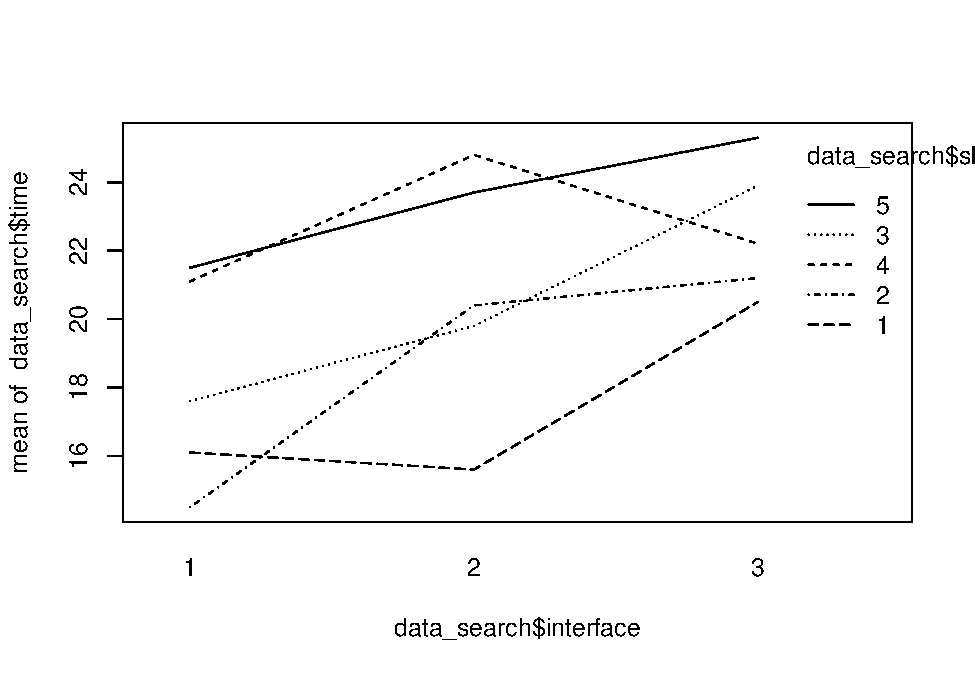
\includegraphics{Assignment-2_files/figure-latex/unnamed-chunk-9-1.pdf}

As shown in the above QQ-plot and the residuals-fitted plot there are
some outliers (points 2, 6, 14) that raise doubt about the normality of
the data. There seems to be some relationship visible, albeit small, in
the Residuals vs Fitted plot - it would be a good idea to perform an
extra test suitable for non-normal data.

\textbf{d)} Perform the Friedman test to test whether there is an effect
of interface.

\begin{Shaded}
\begin{Highlighting}[]
\FunctionTok{friedman.test}\NormalTok{(data\_search}\SpecialCharTok{$}\NormalTok{time, data\_search}\SpecialCharTok{$}\NormalTok{interface, data\_search}\SpecialCharTok{$}\NormalTok{skill)}\SpecialCharTok{$}\NormalTok{p.value}
\end{Highlighting}
\end{Shaded}

\begin{verbatim}
## [1] 0.0408
\end{verbatim}

The test shows a p-value \textless{} 0.05 which is significant. This
means that the \(H_0\) can be rejected and we can state that there is a
significant effect of the interface.

\textbf{e)} Test the null hypothesis that the search time is the same
for all interfaces by a one-way ANOVA test, ignoring the variable skill.
Is it right/wrong or useful/not useful to perform this test on this
dataset?

\begin{Shaded}
\begin{Highlighting}[]
\FunctionTok{anova}\NormalTok{(}\FunctionTok{lm}\NormalTok{(data\_search}\SpecialCharTok{$}\NormalTok{time}\SpecialCharTok{\textasciitilde{}}\NormalTok{data\_search}\SpecialCharTok{$}\NormalTok{interface))}
\end{Highlighting}
\end{Shaded}

\begin{verbatim}
## Analysis of Variance Table
## 
## Response: data_search$time
##                       Df Sum Sq Mean Sq F value Pr(>F)  
## data_search$interface  2   50.5   25.23    2.86  0.096 .
## Residuals             12  105.9    8.82                 
## ---
## Signif. codes:  0 '***' 0.001 '**' 0.01 '*' 0.05 '.' 0.1 ' ' 1
\end{verbatim}

Looking at the p-value (\textgreater{} 0.05) of the one-way ANOVA test,
we see that it is not significant. We could therefore conclude that the
interfaces does not have a significant effect on the search time.
However, since the data originates from a randomised block design, it is
not correct to use this test since it leaves out important effects of
the skill level, which we observed to be significant in \(b)\) and
\(d)\).

\hypertarget{excercise-3}{%
\section{Excercise 3}\label{excercise-3}}

\textbf{a)} Test whether the type of feedingstuffs influences milk
production using an ordinary ``fixed effects'' model, fitted with lm.
Estimate the difference in milk production.

\begin{Shaded}
\begin{Highlighting}[]
\CommentTok{\# read data}
\NormalTok{data }\OtherTok{\textless{}{-}} \FunctionTok{read.table}\NormalTok{(}\AttributeTok{file=}\StringTok{"data/cow.txt"}\NormalTok{,}\AttributeTok{header=}\ConstantTok{TRUE}\NormalTok{)}
\NormalTok{data}\SpecialCharTok{$}\NormalTok{treatment }\OtherTok{\textless{}{-}} \FunctionTok{as.factor}\NormalTok{(data}\SpecialCharTok{$}\NormalTok{treatment); data}\SpecialCharTok{$}\NormalTok{order }\OtherTok{\textless{}{-}} \FunctionTok{as.factor}\NormalTok{(data}\SpecialCharTok{$}\NormalTok{order)}
\NormalTok{data}\SpecialCharTok{$}\NormalTok{id }\OtherTok{\textless{}{-}} \FunctionTok{as.factor}\NormalTok{(data}\SpecialCharTok{$}\NormalTok{id); data}\SpecialCharTok{$}\NormalTok{per }\OtherTok{\textless{}{-}} \FunctionTok{as.factor}\NormalTok{(data}\SpecialCharTok{$}\NormalTok{per)}
\CommentTok{\# perform fixed effects model analysis}
\NormalTok{fixed\_aov }\OtherTok{\textless{}{-}} \FunctionTok{lm}\NormalTok{(milk }\SpecialCharTok{\textasciitilde{}}\NormalTok{ id }\SpecialCharTok{+}\NormalTok{ per }\SpecialCharTok{+}\NormalTok{ treatment, }\AttributeTok{data =}\NormalTok{ data)}
\FunctionTok{anova}\NormalTok{(fixed\_aov); table }\OtherTok{\textless{}{-}} \FunctionTok{summary}\NormalTok{(fixed\_aov)}\SpecialCharTok{$}\NormalTok{coefficients[}\StringTok{"treatmentB"}\NormalTok{,]}
\end{Highlighting}
\end{Shaded}

\begin{verbatim}
## Analysis of Variance Table
## 
## Response: milk
##           Df Sum Sq Mean Sq F value  Pr(>F)    
## id         8   2467   308.4  124.48 7.5e-07 ***
## per        1     25    24.5    9.89   0.016 *  
## treatment  1      1     1.2    0.47   0.517    
## Residuals  7     17     2.5                    
## ---
## Signif. codes:  0 '***' 0.001 '**' 0.01 '*' 0.05 '.' 0.1 ' ' 1
\end{verbatim}

\begin{Shaded}
\begin{Highlighting}[]
\FunctionTok{print}\NormalTok{(}\StringTok{"Estimate for Treatment B:"}\NormalTok{); table}
\end{Highlighting}
\end{Shaded}

\begin{verbatim}
## [1] "Estimate for Treatment B:"
\end{verbatim}

\begin{verbatim}
##   Estimate Std. Error    t value   Pr(>|t|) 
##     -0.510      0.747     -0.683      0.517
\end{verbatim}

From the results of the fixed effects model above we see that the
p-value for treatment is \textgreater{} 0.05, therefore we can conclude
that there is no significant effect of the treatment. From the estimate
of TreatmentB we see that \(\beta_{treatment_B}\) = -0.51 (meaning that
with treatment B we have 0.51 less milk production than with treatment
A), however p-value \textgreater{} 0.05 and, therefore, the difference
is insignificant. However, this model is not correct as it does not take
into consideration the ``random effects'' introduced by the order of the
types of food randomization over the cows.

\textbf{b)} Repeat a) by performing a mixed effects analysis, modelling
the cow effect as a random effect (use the function lmer). Compare your
results to the results found by using a mixed effects model.

\begin{Shaded}
\begin{Highlighting}[]
\FunctionTok{attach}\NormalTok{(data)}
\NormalTok{mixed\_avo }\OtherTok{\textless{}{-}} \FunctionTok{lmer}\NormalTok{(milk }\SpecialCharTok{\textasciitilde{}}\NormalTok{ treatment }\SpecialCharTok{+}\NormalTok{ order }\SpecialCharTok{+}\NormalTok{ per }\SpecialCharTok{+}\NormalTok{ (}\DecValTok{1}\SpecialCharTok{|}\NormalTok{id),}\AttributeTok{REML=}\ConstantTok{FALSE}\NormalTok{); }\FunctionTok{summary}\NormalTok{(mixed\_avo);}
\end{Highlighting}
\end{Shaded}

\begin{verbatim}
## Linear mixed model fit by maximum likelihood  ['lmerMod']
## Formula: milk ~ treatment + order + per + (1 | id)
## 
##      AIC      BIC   logLik deviance df.resid 
##    119.3    124.7    -53.7    107.3       12 
## 
## Scaled residuals: 
##     Min      1Q  Median      3Q     Max 
## -1.5311 -0.3710  0.0269  0.2675  1.7249 
## 
## Random effects:
##  Groups   Name        Variance Std.Dev.
##  id       (Intercept) 133.15   11.54   
##  Residual               1.93    1.39   
## Number of obs: 18, groups:  id, 9
## 
## Fixed effects:
##             Estimate Std. Error t value
## (Intercept)   38.500      5.811    6.63
## treatmentB    -0.510      0.658   -0.77
## orderBA       -3.470      7.768   -0.45
## per2          -2.390      0.658   -3.63
## 
## Correlation of Fixed Effects:
##            (Intr) trtmnB ordrBA
## treatmentB -0.063              
## orderBA    -0.743  0.000       
## per2       -0.063  0.111  0.000
\end{verbatim}

\begin{Shaded}
\begin{Highlighting}[]
\NormalTok{mixed\_avo\_1 }\OtherTok{\textless{}{-}} \FunctionTok{lmer}\NormalTok{(milk }\SpecialCharTok{\textasciitilde{}}\NormalTok{ order }\SpecialCharTok{+}\NormalTok{ per }\SpecialCharTok{+}\NormalTok{ (}\DecValTok{1}\SpecialCharTok{|}\NormalTok{id),}\AttributeTok{REML=}\ConstantTok{FALSE}\NormalTok{)}
\FunctionTok{anova}\NormalTok{(mixed\_avo\_1, mixed\_avo)}
\end{Highlighting}
\end{Shaded}

\begin{verbatim}
## Data: NULL
## Models:
## mixed_avo_1: milk ~ order + per + (1 | id)
## mixed_avo: milk ~ treatment + order + per + (1 | id)
##             npar AIC BIC logLik deviance Chisq Df Pr(>Chisq)
## mixed_avo_1    5 118 122  -53.9      108                    
## mixed_avo      6 119 125  -53.7      107  0.58  1       0.45
\end{verbatim}

The code above implemented the correct model that modeled the cows as
``random effects''. The fixed effects estimates in the summary table are
the same as with the model in a). Furthermore, the code above performed
an ANOVA test between the random effect model with and without treatment
in it. The p-value for treatment is lower with this model than in a),
however it is still \textgreater{} 0.05 - meaning, that there is no
significant difference between the models of with and without treatment,
therefore there is no significant effect of the treatment.

\textbf{c)} Study the commands below. Does this produce a valid test for
a difference in milk production? Is its conclusion compatible with the
one obtained in a)? Why?

\begin{Shaded}
\begin{Highlighting}[]
\FunctionTok{t.test}\NormalTok{(milk[treatment}\SpecialCharTok{==}\StringTok{"A"}\NormalTok{],milk[treatment}\SpecialCharTok{==}\StringTok{"B"}\NormalTok{], }\AttributeTok{paired=}\ConstantTok{TRUE}\NormalTok{)}\SpecialCharTok{$}\NormalTok{p.value}
\end{Highlighting}
\end{Shaded}

\begin{verbatim}
## [1] 0.828
\end{verbatim}

The code above performed a paired t-test (different treatment was done
on the same cow) to test whether the means of the two populations are
significantly different. Here, we see that p-value is \textgreater{}
0.05, which brings us to the same conclusion as with a) and b). However,
this is not correct as we can see from the previous analysis that the
order had a significant effect on the experimental outcomes - a factor
this t-test omits. This t-test is the same as performing a two-way ANOVA
of treament + id. We can see that the p-value is the same:

\begin{Shaded}
\begin{Highlighting}[]
\FunctionTok{paste}\NormalTok{(}\StringTok{"p{-}value with two{-}way ANOVA:"}\NormalTok{, }
      \FunctionTok{round}\NormalTok{(}\FunctionTok{anova}\NormalTok{(}\FunctionTok{lm}\NormalTok{(milk }\SpecialCharTok{\textasciitilde{}}\NormalTok{ treatment }\SpecialCharTok{+}\NormalTok{ id, }\AttributeTok{data =}\NormalTok{ data))[}\StringTok{"treatment"}\NormalTok{, ]}\SpecialCharTok{$}\StringTok{\textasciigrave{}}\AttributeTok{Pr(\textgreater{}F)}\StringTok{\textasciigrave{}}\NormalTok{, }\DecValTok{3}\NormalTok{))}
\end{Highlighting}
\end{Shaded}

\begin{verbatim}
## [1] "p-value with two-way ANOVA: 0.828"
\end{verbatim}

\hypertarget{exercise-4}{%
\section{Exercise 4}\label{exercise-4}}

\textbf{a)} Discuss whether a contingency table test for independence or
for homogeneity is most appropriate here.

The contingency table test for homogeneity is appropriate because we
want to know if the fan writer imitates Austen in a good way. This means
that we want to test whether or not the different columns of data in the
table come from the same population (writer) or not, which would be the
case it the fan imitated Austen correctly. The \(H_0\) of the
contingency table test for homogeneity states that the distribution of
the words is the same for the stories.

\textbf{b)} Using the given data set, investigate whether Austen herself
was consistent in her different novels. Where are the main
inconsistencies?

\begin{Shaded}
\begin{Highlighting}[]
\NormalTok{data }\OtherTok{\textless{}{-}} \FunctionTok{read.table}\NormalTok{(}\AttributeTok{file=}\StringTok{"data/austen.txt"}\NormalTok{,}\AttributeTok{header=}\ConstantTok{TRUE}\NormalTok{)}
\NormalTok{austen }\OtherTok{\textless{}{-}}\NormalTok{ data[,}\DecValTok{1}\SpecialCharTok{:}\DecValTok{3}\NormalTok{] }\CommentTok{\# filter data to only have data from Austen}
\NormalTok{z }\OtherTok{=} \FunctionTok{chisq.test}\NormalTok{(austen); z; }\FunctionTok{residuals}\NormalTok{(z)}
\end{Highlighting}
\end{Shaded}

\begin{verbatim}
## 
##  Pearson's Chi-squared test
## 
## data:  austen
## X-squared = 12, df = 10, p-value = 0.3
\end{verbatim}

\begin{verbatim}
##           Sense   Emma  Sand1
## a       -1.0300 -0.129  1.594
## an       0.4473 -0.159 -0.375
## this     0.0513  0.294 -0.504
## that     0.7482  0.287 -1.442
## with    -0.0475  0.521 -0.704
## without  1.0654 -1.588  0.893
\end{verbatim}

She is not inconsistent as the p-value is above 0.05. This means that we
cannot reject the \(H_0\). She does however, have some main
inconsistency, which are the words ``a'', ``that'' and ``without'' - as
can be seen in the residual table above.

\textbf{c)} Was the admirer successful in imitating Austen's style?
Perform a test including all data. If he was not successful, where are
the differences?

\begin{Shaded}
\begin{Highlighting}[]
\NormalTok{z }\OtherTok{=} \FunctionTok{chisq.test}\NormalTok{(data); z; }\FunctionTok{residuals}\NormalTok{(z)}
\end{Highlighting}
\end{Shaded}

\begin{verbatim}
## 
##  Pearson's Chi-squared test
## 
## data:  data
## X-squared = 46, df = 15, p-value = 6e-05
\end{verbatim}

\begin{verbatim}
##          Sense      Emma  Sand1   Sand2
## a       -1.015 -0.112093  1.606 -0.0589
## an      -0.591 -1.219955 -1.067  3.7282
## this     0.139  0.390490 -0.444 -0.3267
## that     1.594  1.179849 -0.910 -3.0493
## with    -0.512  0.000192 -1.025  1.7482
## without  1.392 -1.341196  1.137 -1.0696
\end{verbatim}

The fan is inconsistent as the p-value of the test is below 0.05.
Therefore, we have to reject the \(H_0\) and accept that the
distribution of the words in the stories are not the same. Because
Austen herself did not have this inconsistency we can say that the
inconsistency is caused by the fan writer. The main inconsistencies were
for the words ``that'' and ``an''. As can be seen in the residual table
above.

\hypertarget{exercise-5}{%
\section{Exercise 5}\label{exercise-5}}

\textbf{a)} Make some graphical summaries of the data. Investigate the
problem of potential and influence points,and the problem of
collinearity.

\begin{Shaded}
\begin{Highlighting}[]
\NormalTok{data\_crime }\OtherTok{=} \FunctionTok{read.table}\NormalTok{(}\AttributeTok{file=}\StringTok{"data/expensescrime.txt"}\NormalTok{,}\AttributeTok{header=}\ConstantTok{TRUE}\NormalTok{)}
\NormalTok{regression\_data }\OtherTok{=}\NormalTok{ data\_crime[}\DecValTok{2}\SpecialCharTok{:}\DecValTok{7}\NormalTok{]; }\FunctionTok{pairs}\NormalTok{(regression\_data)}
\end{Highlighting}
\end{Shaded}

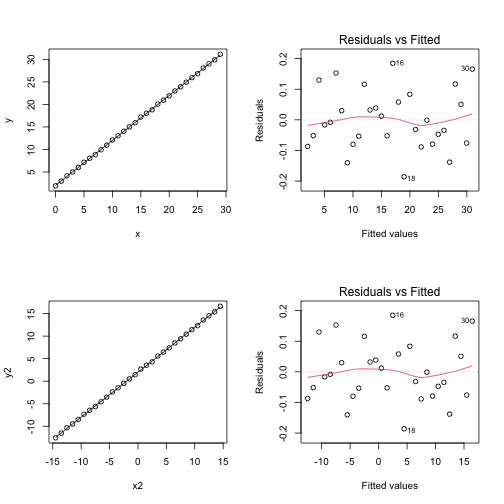
\includegraphics{Assignment-2_files/figure-latex/unnamed-chunk-18-1.pdf}
From the pairs plot above we can clearly see linear relationships
between predictors \(bad\), \(lawyer\), \(employ\) and \(pop\) - this
could cause a problem of collinearity. Looking at predictors vs
\(expend\) we can see a strong linear relationship with \(bad\),
\(lawyers\), \(employ\) and \(pop\); no obvious relationship can be
observed with \(crime\).

\textbf{\emph{Influence points}}

\begin{Shaded}
\begin{Highlighting}[]
\NormalTok{cooks\_crime }\OtherTok{\textless{}{-}} \FunctionTok{cooks.distance}\NormalTok{(}\FunctionTok{lm}\NormalTok{(expend}\SpecialCharTok{\textasciitilde{}}\NormalTok{crime }\SpecialCharTok{+}\NormalTok{ bad }\SpecialCharTok{+}\NormalTok{ lawyers }\SpecialCharTok{+}\NormalTok{ employ }\SpecialCharTok{+}\NormalTok{ pop, }
                                 \AttributeTok{data =}\NormalTok{ regression\_data))}
\FunctionTok{plot}\NormalTok{(cooks\_crime, }\AttributeTok{type=}\StringTok{"b"}\NormalTok{);}
\end{Highlighting}
\end{Shaded}

\includegraphics{Assignment-2_files/figure-latex/unnamed-chunk-19-1.pdf}

\begin{Shaded}
\begin{Highlighting}[]
\CommentTok{\# remove influence points from the data}
\NormalTok{remove }\OtherTok{\textless{}{-}} \FunctionTok{which}\NormalTok{(cooks\_crime }\SpecialCharTok{\textgreater{}} \DecValTok{1}\NormalTok{); }
\NormalTok{regression\_data }\OtherTok{\textless{}{-}}\NormalTok{ regression\_data }\SpecialCharTok{\%\textgreater{}\%} \FunctionTok{mutate}\NormalTok{(}\AttributeTok{row\_n =} \FunctionTok{row\_number}\NormalTok{()) }\SpecialCharTok{\%\textgreater{}\%}
  \FunctionTok{filter}\NormalTok{(}\SpecialCharTok{!}\NormalTok{(row\_n }\SpecialCharTok{\%in\%}\NormalTok{ remove)) }\SpecialCharTok{\%\textgreater{}\%} \FunctionTok{select}\NormalTok{(}\SpecialCharTok{{-}}\NormalTok{row\_n)}
\end{Highlighting}
\end{Shaded}

Model containing all of predictors was chosen to find influence points
as we have not yet selected which predictors will be used in the final
model. From the figure above we can see that points 5, 8, 35 and 44 have
Cook's distance of \textgreater{} 1, therefore they were regarded as
influence points and removed from the data.

\textbf{\emph{Collinearity}}

\begin{Shaded}
\begin{Highlighting}[]
\NormalTok{knitr}\SpecialCharTok{::}\FunctionTok{kable}\NormalTok{(}\FunctionTok{round}\NormalTok{(}\FunctionTok{cor}\NormalTok{(regression\_data),}\DecValTok{2}\NormalTok{), }\AttributeTok{caption =} \StringTok{"Correlation coefficients"}\NormalTok{)}
\end{Highlighting}
\end{Shaded}

\begin{longtable}[]{@{}lrrrrrr@{}}
\caption{Correlation coefficients}\tabularnewline
\toprule
& expend & bad & crime & lawyers & employ & pop\tabularnewline
\midrule
\endfirsthead
\toprule
& expend & bad & crime & lawyers & employ & pop\tabularnewline
\midrule
\endhead
expend & 1.00 & 0.90 & 0.34 & 0.96 & 0.98 & 0.96\tabularnewline
bad & 0.90 & 1.00 & 0.33 & 0.85 & 0.90 & 0.91\tabularnewline
crime & 0.34 & 0.33 & 1.00 & 0.25 & 0.25 & 0.18\tabularnewline
lawyers & 0.96 & 0.85 & 0.25 & 1.00 & 0.97 & 0.95\tabularnewline
employ & 0.98 & 0.90 & 0.25 & 0.97 & 1.00 & 0.97\tabularnewline
pop & 0.96 & 0.91 & 0.18 & 0.95 & 0.97 & 1.00\tabularnewline
\bottomrule
\end{longtable}

Correlation table above produced results similar to what was observer
with pairs plot before - we see that (excluding variable \(crime\)), the
lowest correlation coefficient is 0.85 (between \(bad\) and
\(lawyers\)), which is still a high correlation coefficient. This means
that all predictors (excluding \(crime\)) carry similar information.

\textbf{b)} Fit a linear regression model to the data. Use both the
step-up and the step-down method to find the best model. If step-up and
step-down yield two different models, choose one and motivate your
choice.

\textbf{\emph{Step-up method:}}

\begin{Shaded}
\begin{Highlighting}[]
\CommentTok{\# level 1}
\NormalTok{model\_bad }\OtherTok{\textless{}{-}} \FunctionTok{lm}\NormalTok{(expend}\SpecialCharTok{\textasciitilde{}}\NormalTok{bad, }\AttributeTok{data=}\NormalTok{regression\_data); }
\NormalTok{model\_crime }\OtherTok{\textless{}{-}} \FunctionTok{lm}\NormalTok{(expend}\SpecialCharTok{\textasciitilde{}}\NormalTok{crime, }\AttributeTok{data=}\NormalTok{regression\_data)}
\NormalTok{model\_lawyers }\OtherTok{\textless{}{-}} \FunctionTok{lm}\NormalTok{(expend}\SpecialCharTok{\textasciitilde{}}\NormalTok{lawyers, }\AttributeTok{data=}\NormalTok{regression\_data); }
\NormalTok{model\_employ }\OtherTok{\textless{}{-}} \FunctionTok{lm}\NormalTok{(expend}\SpecialCharTok{\textasciitilde{}}\NormalTok{employ, }\AttributeTok{data=}\NormalTok{regression\_data)}
\NormalTok{model\_pop }\OtherTok{\textless{}{-}} \FunctionTok{lm}\NormalTok{(expend}\SpecialCharTok{\textasciitilde{}}\NormalTok{pop, }\AttributeTok{data=}\NormalTok{regression\_data)}
\NormalTok{level1\_models }\OtherTok{\textless{}{-}} \FunctionTok{list}\NormalTok{(model\_bad, model\_crime, model\_employ, model\_lawyers, model\_pop); }
\NormalTok{variables\_1 }\OtherTok{\textless{}{-}} \FunctionTok{c}\NormalTok{(}\StringTok{"bad"}\NormalTok{, }\StringTok{"crime"}\NormalTok{, }\StringTok{"employ"}\NormalTok{, }\StringTok{"lawyears"}\NormalTok{, }\StringTok{"pop"}\NormalTok{)}

\NormalTok{r\_squared\_values\_1 }\OtherTok{\textless{}{-}} \FunctionTok{c}\NormalTok{()}
\ControlFlowTok{for}\NormalTok{(model\_1 }\ControlFlowTok{in}\NormalTok{ level1\_models)\{}
\NormalTok{  r\_squared }\OtherTok{\textless{}{-}}  \FunctionTok{summary}\NormalTok{(model\_1)}\SpecialCharTok{$}\NormalTok{r.squared}
\NormalTok{  r\_squared\_values\_1 }\OtherTok{\textless{}{-}} \FunctionTok{c}\NormalTok{(r\_squared\_values\_1, r\_squared)}
\NormalTok{\}}

\NormalTok{knitr}\SpecialCharTok{::}\FunctionTok{kable}\NormalTok{(}\FunctionTok{data.frame}\NormalTok{(}\AttributeTok{Predictor =}\NormalTok{ variables\_1, }\AttributeTok{r.squared =}\NormalTok{ r\_squared\_values\_1) }\SpecialCharTok{\%\textgreater{}\%}
               \FunctionTok{mutate}\NormalTok{(}\AttributeTok{Selected =} \FunctionTok{if\_else}\NormalTok{(r.squared }\SpecialCharTok{==} \FunctionTok{max}\NormalTok{(r.squared),}\StringTok{"Yes"}\NormalTok{, }\StringTok{"No"}\NormalTok{)), }
             \AttributeTok{caption =} \StringTok{"Step{-}up: Level 1"}\NormalTok{)}
\end{Highlighting}
\end{Shaded}

\begin{longtable}[]{@{}lrl@{}}
\caption{Step-up: Level 1}\tabularnewline
\toprule
Predictor & r.squared & Selected\tabularnewline
\midrule
\endfirsthead
\toprule
Predictor & r.squared & Selected\tabularnewline
\midrule
\endhead
bad & 0.817 & No\tabularnewline
crime & 0.117 & No\tabularnewline
employ & 0.955 & Yes\tabularnewline
lawyears & 0.927 & No\tabularnewline
pop & 0.930 & No\tabularnewline
\bottomrule
\end{longtable}

\begin{Shaded}
\begin{Highlighting}[]
\CommentTok{\# level 2}
\NormalTok{model\_bad\_2 }\OtherTok{\textless{}{-}} \FunctionTok{lm}\NormalTok{(expend}\SpecialCharTok{\textasciitilde{}}\NormalTok{employ}\SpecialCharTok{+}\NormalTok{bad, }\AttributeTok{data=}\NormalTok{regression\_data); }
\NormalTok{model\_crime\_2 }\OtherTok{\textless{}{-}} \FunctionTok{lm}\NormalTok{(expend}\SpecialCharTok{\textasciitilde{}}\NormalTok{employ}\SpecialCharTok{+}\NormalTok{crime, }\AttributeTok{data=}\NormalTok{regression\_data)}
\NormalTok{model\_pop\_2 }\OtherTok{\textless{}{-}} \FunctionTok{lm}\NormalTok{(expend}\SpecialCharTok{\textasciitilde{}}\NormalTok{employ}\SpecialCharTok{+}\NormalTok{pop, }\AttributeTok{data=}\NormalTok{regression\_data); }
\NormalTok{model\_lawyers\_2 }\OtherTok{\textless{}{-}} \FunctionTok{lm}\NormalTok{(expend}\SpecialCharTok{\textasciitilde{}}\NormalTok{employ}\SpecialCharTok{+}\NormalTok{lawyers, }\AttributeTok{data=}\NormalTok{regression\_data)}
\NormalTok{level2\_models }\OtherTok{\textless{}{-}} \FunctionTok{list}\NormalTok{(model\_bad\_2, model\_crime\_2, model\_lawyers\_2, model\_pop\_2); }
\NormalTok{variables\_2 }\OtherTok{\textless{}{-}} \FunctionTok{c}\NormalTok{(}\StringTok{"employ+bad"}\NormalTok{, }\StringTok{"employ+crime"}\NormalTok{, }\StringTok{"employ+lawyears"}\NormalTok{, }\StringTok{"employ+pop"}\NormalTok{)}

\NormalTok{r\_squared\_values\_2 }\OtherTok{\textless{}{-}} \FunctionTok{c}\NormalTok{()}
\NormalTok{significance\_2 }\OtherTok{\textless{}{-}} \FunctionTok{c}\NormalTok{()}
\ControlFlowTok{for}\NormalTok{(model\_1 }\ControlFlowTok{in}\NormalTok{ level2\_models)\{}
\NormalTok{  is\_significant }\OtherTok{\textless{}{-}} \FunctionTok{sum}\NormalTok{(}\FunctionTok{c}\NormalTok{(}\FunctionTok{summary}\NormalTok{(model\_1)}\SpecialCharTok{$}\NormalTok{coefficients[,}\DecValTok{4}\NormalTok{] }\SpecialCharTok{\textless{}} \FloatTok{0.05}\NormalTok{)) }\SpecialCharTok{\textgreater{}} \DecValTok{2} 
\NormalTok{  r\_squared }\OtherTok{\textless{}{-}}  \FunctionTok{summary}\NormalTok{(model\_1)}\SpecialCharTok{$}\NormalTok{r.squared}
\NormalTok{  r\_squared\_values\_2 }\OtherTok{\textless{}{-}} \FunctionTok{c}\NormalTok{(r\_squared\_values\_2, r\_squared)}
\NormalTok{  significance\_2 }\OtherTok{\textless{}{-}} \FunctionTok{c}\NormalTok{(significance\_2, is\_significant) }
\NormalTok{\}}

\NormalTok{knitr}\SpecialCharTok{::}\FunctionTok{kable}\NormalTok{(}\FunctionTok{data.frame}\NormalTok{(}\AttributeTok{Predictor =}\NormalTok{ variables\_2, }\AttributeTok{r.squared =}\NormalTok{ r\_squared\_values\_2, }
  \AttributeTok{Significant =}\NormalTok{ significance\_2) }\SpecialCharTok{\%\textgreater{}\%} \FunctionTok{mutate}\NormalTok{(}\AttributeTok{Selected =} \FunctionTok{if\_else}\NormalTok{(Significant,}\StringTok{"Yes"}\NormalTok{, }\StringTok{"No"}\NormalTok{)), }
  \AttributeTok{caption =} \StringTok{"Step{-}up: Level 2"}\NormalTok{)}
\end{Highlighting}
\end{Shaded}

\begin{longtable}[]{@{}lrll@{}}
\caption{Step-up: Level 2}\tabularnewline
\toprule
Predictor & r.squared & Significant & Selected\tabularnewline
\midrule
\endfirsthead
\toprule
Predictor & r.squared & Significant & Selected\tabularnewline
\midrule
\endhead
employ+bad & 0.957 & FALSE & No\tabularnewline
employ+crime & 0.964 & TRUE & Yes\tabularnewline
employ+lawyears & 0.960 & FALSE & No\tabularnewline
employ+pop & 0.960 & FALSE & No\tabularnewline
\bottomrule
\end{longtable}

\begin{Shaded}
\begin{Highlighting}[]
\CommentTok{\# level 3}

\NormalTok{model\_bad\_3 }\OtherTok{\textless{}{-}} \FunctionTok{lm}\NormalTok{(expend}\SpecialCharTok{\textasciitilde{}}\NormalTok{employ}\SpecialCharTok{+}\NormalTok{crime}\SpecialCharTok{+}\NormalTok{bad, }\AttributeTok{data=}\NormalTok{regression\_data);}
\NormalTok{model\_pop\_3 }\OtherTok{\textless{}{-}} \FunctionTok{lm}\NormalTok{(expend}\SpecialCharTok{\textasciitilde{}}\NormalTok{employ}\SpecialCharTok{+}\NormalTok{crime}\SpecialCharTok{+}\NormalTok{pop, }\AttributeTok{data=}\NormalTok{regression\_data);}
\NormalTok{model\_lawyers\_3 }\OtherTok{\textless{}{-}} \FunctionTok{lm}\NormalTok{(expend}\SpecialCharTok{\textasciitilde{}}\NormalTok{employ}\SpecialCharTok{+}\NormalTok{crime}\SpecialCharTok{+}\NormalTok{lawyers, }\AttributeTok{data=}\NormalTok{regression\_data);}
\NormalTok{level3\_models }\OtherTok{\textless{}{-}} \FunctionTok{list}\NormalTok{(model\_bad\_3, model\_lawyers\_3, model\_pop\_3); }
\NormalTok{variables\_3 }\OtherTok{\textless{}{-}} \FunctionTok{c}\NormalTok{(}\StringTok{"employ+crime+bad"}\NormalTok{, }\StringTok{"employ+crime+lawyers"}\NormalTok{, }\StringTok{"employ+crime+pop"}\NormalTok{)}

\NormalTok{r\_squared\_values\_3 }\OtherTok{\textless{}{-}} \FunctionTok{c}\NormalTok{()}
\NormalTok{significance\_3 }\OtherTok{\textless{}{-}} \FunctionTok{c}\NormalTok{()}
\ControlFlowTok{for}\NormalTok{(model\_1 }\ControlFlowTok{in}\NormalTok{ level3\_models)\{}
\NormalTok{  is\_significant }\OtherTok{\textless{}{-}} \FunctionTok{sum}\NormalTok{(}\FunctionTok{c}\NormalTok{(}\FunctionTok{summary}\NormalTok{(model\_1)}\SpecialCharTok{$}\NormalTok{coefficients[,}\DecValTok{4}\NormalTok{] }\SpecialCharTok{\textless{}} \FloatTok{0.05}\NormalTok{)) }\SpecialCharTok{\textgreater{}} \DecValTok{3} 
\NormalTok{  r\_squared }\OtherTok{\textless{}{-}}  \FunctionTok{summary}\NormalTok{(model\_1)}\SpecialCharTok{$}\NormalTok{r.squared}
\NormalTok{  r\_squared\_values\_3 }\OtherTok{\textless{}{-}} \FunctionTok{c}\NormalTok{(r\_squared\_values\_3, r\_squared)}
\NormalTok{  significance\_3 }\OtherTok{\textless{}{-}} \FunctionTok{c}\NormalTok{(significance\_3, is\_significant) }
\NormalTok{\}}

\NormalTok{knitr}\SpecialCharTok{::}\FunctionTok{kable}\NormalTok{(}\FunctionTok{data.frame}\NormalTok{(}\AttributeTok{Predictor =}\NormalTok{ variables\_3, }\AttributeTok{r.squared =}\NormalTok{ r\_squared\_values\_3, }
  \AttributeTok{Significant =}\NormalTok{ significance\_3) }\SpecialCharTok{\%\textgreater{}\%} 
    \FunctionTok{mutate}\NormalTok{(}\AttributeTok{Selected =} \FunctionTok{if\_else}\NormalTok{(Significant }\SpecialCharTok{\&}\NormalTok{ r.squared }\SpecialCharTok{==} \FunctionTok{max}\NormalTok{(r.squared),}\StringTok{"Yes"}\NormalTok{, }\StringTok{"No"}\NormalTok{)), }
  \AttributeTok{caption =} \StringTok{"Step{-}up: Level 3"}\NormalTok{)}
\end{Highlighting}
\end{Shaded}

\begin{longtable}[]{@{}lrll@{}}
\caption{Step-up: Level 3}\tabularnewline
\toprule
Predictor & r.squared & Significant & Selected\tabularnewline
\midrule
\endfirsthead
\toprule
Predictor & r.squared & Significant & Selected\tabularnewline
\midrule
\endhead
employ+crime+bad & 0.965 & FALSE & No\tabularnewline
employ+crime+lawyers & 0.970 & TRUE & No\tabularnewline
employ+crime+pop & 0.974 & TRUE & Yes\tabularnewline
\bottomrule
\end{longtable}

\textbf{\emph{Step up method:}} First we started by fitting a linear
model with one explanatory variable. Out of the 5 available variables
\(employ\) performed the best according to r-squared value, therefore it
was selected for further fitting. Next, another layer of explanatory
variables was added to the linear model. Here, only adding \(crime\)
resulted in a model that had all significant parameters, therefore it
was the model we carried on with. Next, we added a third layer of
variables. \(pop\) seemed to give the best results according to
r-squared values (and also had all significant parameters). However,
looking back at previous analysis, we know that \(pop\) and \(employ\)
are strongly correlated and it would not make sense to have them in the
same model, therefore we performed VIF analysis:

\begin{Shaded}
\begin{Highlighting}[]
\CommentTok{\# VIF analysis}
\FunctionTok{vif}\NormalTok{(model\_pop\_3)}
\end{Highlighting}
\end{Shaded}

\begin{verbatim}
## employ  crime    pop 
##  17.87   1.14  17.31
\end{verbatim}

From the VIF analysis we see that indeed having these two parameters
should be avoided as VIF for them is \textgreater{} 5. We removed
\(pop\) from the model even though it had lower VIF - removing
\(employ\) resulted in lower r-squared value. Removal of this variable
did not have a high impact on the r-squared value as addition of it only
brought marginal improvement. VIF of the model without \(pop\) (as seen
below) is now acceptable:

\begin{Shaded}
\begin{Highlighting}[]
\FunctionTok{vif}\NormalTok{(model\_crime\_2)}
\end{Highlighting}
\end{Shaded}

\begin{verbatim}
## employ  crime 
##   1.07   1.07
\end{verbatim}

Therefore, the final model from the step-up method is as follows:

\begin{Shaded}
\begin{Highlighting}[]
\FunctionTok{summary}\NormalTok{(model\_crime\_2)}\SpecialCharTok{$}\NormalTok{coefficients}
\end{Highlighting}
\end{Shaded}

\begin{verbatim}
##              Estimate Std. Error t value Pr(>|t|)
## (Intercept) -165.9828   59.78132   -2.78 8.11e-03
## employ         0.0363    0.00113   31.96 1.33e-31
## crime          0.0432    0.01280    3.38 1.57e-03
\end{verbatim}

\(expend = -165.9828 + 0.0363 \times employ + 0.0432 \times crime + error\)

\textbf{\emph{Step-down method:}}

\begin{Shaded}
\begin{Highlighting}[]
\CommentTok{\# step down method {-} start with all}
\FunctionTok{summary}\NormalTok{(}\FunctionTok{lm}\NormalTok{(expend}\SpecialCharTok{\textasciitilde{}}\NormalTok{bad}\SpecialCharTok{+}\NormalTok{crime}\SpecialCharTok{+}\NormalTok{lawyers}\SpecialCharTok{+}\NormalTok{employ}\SpecialCharTok{+}\NormalTok{pop, }\AttributeTok{data=}\NormalTok{regression\_data))}\SpecialCharTok{$}\NormalTok{coefficients}
\end{Highlighting}
\end{Shaded}

\begin{verbatim}
##              Estimate Std. Error t value Pr(>|t|)
## (Intercept) -241.6684   60.15675 -4.0173 0.000252
## bad           -0.0321    0.94970 -0.0338 0.973216
## crime          0.0531    0.01214  4.3772 0.000084
## lawyers        0.0118    0.00659  1.7888 0.081216
## employ         0.0162    0.00481  3.3606 0.001720
## pop            0.0625    0.02100  2.9765 0.004930
\end{verbatim}

\begin{Shaded}
\begin{Highlighting}[]
\CommentTok{\# remove bad}
\FunctionTok{summary}\NormalTok{(}\FunctionTok{lm}\NormalTok{(expend}\SpecialCharTok{\textasciitilde{}}\NormalTok{crime}\SpecialCharTok{+}\NormalTok{lawyers}\SpecialCharTok{+}\NormalTok{employ}\SpecialCharTok{+}\NormalTok{pop, }\AttributeTok{data=}\NormalTok{regression\_data))}\SpecialCharTok{$}\NormalTok{coefficients}
\end{Highlighting}
\end{Shaded}

\begin{verbatim}
##              Estimate Std. Error t value Pr(>|t|)
## (Intercept) -240.8488   54.37368   -4.43 6.87e-05
## crime          0.0530    0.01106    4.79 2.21e-05
## lawyers        0.0119    0.00615    1.93 6.03e-02
## employ         0.0161    0.00454    3.55 9.79e-04
## pop            0.0622    0.01836    3.39 1.57e-03
\end{verbatim}

\begin{Shaded}
\begin{Highlighting}[]
\CommentTok{\# remove lawyers}
\FunctionTok{summary}\NormalTok{(}\FunctionTok{lm}\NormalTok{(expend}\SpecialCharTok{\textasciitilde{}}\NormalTok{crime}\SpecialCharTok{+}\NormalTok{employ}\SpecialCharTok{+}\NormalTok{pop, }\AttributeTok{data=}\NormalTok{regression\_data))}\SpecialCharTok{$}\NormalTok{coefficients}
\end{Highlighting}
\end{Shaded}

\begin{verbatim}
##              Estimate Std. Error t value Pr(>|t|)
## (Intercept) -252.6057   55.76140   -4.53 4.82e-05
## crime          0.0548    0.01138    4.81 1.95e-05
## employ         0.0207    0.00399    5.19 5.66e-06
## pop            0.0727    0.01810    4.02 2.40e-04
\end{verbatim}

\textbf{\emph{Step-down method:}} We started with a model that used all
of the available predictors. From the summary table we see that \(bad\)
had the highest (and insignificant) p-value - therefore, it was removed.
Next we see that \(lawyers\) was the only insignificant parameter and
therefore, was removed from the model. The resulting model of
\(crime + employ + pop\) has all significant parameters and is the same
as produced with the step-up method. However, as before, \(pop\) should
be removed as it is colinear with \(employ\).

\textbf{\emph{Conclusion}} Both step-up and step-down methods bring us
to the same model of \(employ + crime\). However, we can see that both
models posses a negative intercept. Conceptually, this does not make
sense as the expenditure of the government can not be negative even if
all of the predictors are 0. Taking this into consideration, in addition
to Occam's razor principle and the fact that introduction of extra
predictor (\(crime\)) to \(employ\) did not bring substantial
improvement to r-squared (only \(\approx\) +0.01) we choose the
following model as the final model:

\begin{Shaded}
\begin{Highlighting}[]
\FunctionTok{summary}\NormalTok{(}\FunctionTok{lm}\NormalTok{(expend}\SpecialCharTok{\textasciitilde{}}\NormalTok{employ, }\AttributeTok{data=}\NormalTok{regression\_data))}\SpecialCharTok{$}\NormalTok{coefficients}
\end{Highlighting}
\end{Shaded}

\begin{verbatim}
##             Estimate Std. Error t value Pr(>|t|)
## (Intercept)  19.1763   26.42996   0.726 4.72e-01
## employ        0.0372    0.00122  30.510 3.07e-31
\end{verbatim}

Even though the intercept parameter is insignificant, it is in principle
not always a problem and could mean that the model starts at the origin.
However, it will not be removed as we do not have enough information to
make a concrete decision on this. The final model is as follows:

\(expend = 19.1763 + 0.0372 \times employ + error\)

\textbf{c)} Check the model assumptions (of the resulting model from b))
by using relevant diagnostic tools.

\begin{Shaded}
\begin{Highlighting}[]
\NormalTok{right\_plot }\OtherTok{=} \FunctionTok{lm}\NormalTok{(expend}\SpecialCharTok{\textasciitilde{}}\NormalTok{employ , }\AttributeTok{data=}\NormalTok{regression\_data)}
\FunctionTok{par}\NormalTok{(}\AttributeTok{mfrow=}\FunctionTok{c}\NormalTok{(}\DecValTok{1}\NormalTok{,}\DecValTok{2}\NormalTok{)); }\FunctionTok{plot}\NormalTok{(right\_plot, }\DecValTok{1}\NormalTok{); }\FunctionTok{plot}\NormalTok{(right\_plot, }\DecValTok{2}\NormalTok{)}
\end{Highlighting}
\end{Shaded}

\includegraphics{Assignment-2_files/figure-latex/unnamed-chunk-27-1.pdf}

From the diagnostic plots above:

\begin{itemize}
\tightlist
\item
  Normal qq-plot: residuals follow a straight line pretty well, however
  there are some outliers at the extremes - removing them could improve
  the results.
\item
  Residuals vs fitted: as desired, there does not seem to be any trend.
\end{itemize}

\end{document}
